\section{Kollaboration}\label{section:konzeption:kollaboration}

\usetikzlibrary{arrows.meta}

Nach \autoref{requirement:Kollaboration} soll die IDE die Echtzeit-Kollaboration mit anderen Laborgeräten innerhalb eines Experiments unterstützen. Dafür soll laut Unteranforderung (a) ein entsprechender CrossLab-Service entwickelt werden. Dieser soll nach Unteranforderung (b) für die Ermöglichung der Echtzeit-Kollaboration von der IDE verwendet werden.

Es gibt viele verschiedene Methoden zur Synchronisierung von Daten zwischen mehreren Teilnehmern. Beispiele derartiger Methoden sind \emph{\ac{OT}} \cite{sun_operational_1998}, \emph{Differential Synchronization} \cite{fraser_differential_2009} und \emph{\acp{CRDT}} \cite{shapiro_conflict-free_2011}. Aufgrund der Tatsache, dass jede dieser Methoden eigene Vor- und Nachteile besitzt, sollte die entwickelte Lösung möglichst unabhängig von dem zugrunde liegenden Synchronisationsalgorithmus sein, damit für den jeweiligen Anwendungsfall der passende Algorithmus verwendet werden kann\todo{Feedback einholen}. Daher werden zunächst die grundlegenden Konzepte beschrieben, bevor der entwickelte CrossLab-Service vorgestellt wird.

Im Folgenden wird für die Erklärung der Konzepte von mehreren an der Kollaboration teilnehmenden Clients und einem zentralen Synchronisationsserver ausgegangen. Die Clients besitzen die Möglichkeit, sogenannte \textit{Räume} zu erstellen bzw. ihnen beizutreten. Jeder Raum verwaltet ein geteiltes Objekt, dabei wird im Folgenden für die Veranschaulichung von einem JSON-Objekt ausgegangen. Dieses nutzt Strings als Schlüssel mit entsprechenden kollaborativen Datentypen als Werten. Kollaborative Datentypen bieten spezielle Methoden zur Bearbeitung dieser an und sind abhängig von der verwendeten Synchronisationsmethode. Im Falle eines JSON-Objekts werden z.B. kollaborative Datentypen für die JSON-Datentypen Object, Array, Number, String, Boolean und Null benötigt. Änderungen an dem geteilten Objekt werden über den zentralen Server an die anderen Teilnehmer weitergeleitet. Zusätzlich können die Clients Zustandsinformationen an den Server melden, welcher diese ebenso an die anderen Clients weiterleitet. Für die Zustandsinformationen können normale Datentypen verwendet werden. Die Zustandsinformationen eines Clients können nur von diesem selbst verändert werden. Außerdem sollten die Clients ihre Zustandsinformationen regelmäßig aktualisieren. Clients können die Zustandsinformationen eines anderen Teilnehmers löschen, falls für eine gewisse Zeit keine Aktualisierung dieser vorgenommen wurde. Dadurch können z.B. Verbindungsabbrüche von Clients behandelt werden. Basierend auf diesen Konzepten wird nachfolgend der \textit{Collaboration Service} anhand bestimmter Szenarien vorgestellt.

\begin{figure}[tbp]
    \centering
    \resizebox{0.9\textwidth}{!}{\begin{sequencediagram}
            \newthread{consumer1}{Consumer 1}
            \newthreadShift{producer}{Producer}{3cm}
            \newthreadShift{consumer2}{Consumer 2}{3cm}

            \begin{call}{consumer1}{trete Räumen bei}{consumer1}{}
            \end{call}
            \prelevel\prelevel
            \begin{call}{consumer2}{trete Räumen bei}{consumer2}{}
            \end{call}

            \begin{call}{consumer1}{Initialisierung}{producer}{}
                \begin{call}{producer}{registriere Consumer}{producer}{}
                \end{call}
            \end{call}
            \begin{call}{consumer1}{starte Synchronisation}{producer}{}
            \end{call}

            \begin{call}{consumer2}{Initialisierung}{producer}{}
                \begin{call}{producer}{registriere Consumer}{producer}{}
                \end{call}
            \end{call}
            \begin{call}{consumer2}{starte Synchronisation}{producer}{}
            \end{call}
        \end{sequencediagram}}
    \caption{Beispiel Initialisierung Synchronisation}
    \label{figure:initialisierung-synchronisation}
\end{figure}

Zunächst wird die Initialisierung der Synchronisation zwischen dem Collaboration Service Producer und dem Collaboration Service Consumer betrachtet. Dafür ist in \autoref{figure:initialisierung-synchronisation} ein möglicher Ablauf dargestellt. Zunächst tritt der Collaboration Service Consumer den Räumen bei, für welche er Daten bereitstellt bzw. welche in der Konfiguration der Verbindung mit dem jeweiligen Producer angegeben wurden. Der Beitritt in Räume kann auch nach dem Beginn der Synchronisation geschehen. Nachdem der Collaboration Service Consumer den Räumen beigetreten ist, sendet dieser eine Initialisierungsnachricht an den Collaboration Service Producer, welche u.a. einen einzigartigen Kennzeichner für den Collaboration Service Consumer beinhaltet. Dieser Kennzeichner kann entweder generiert werden oder über die Konfiguration der entsprechenden Laborgeräte während der Konfiguration des Experiments angegeben werden. Die Informationen der Initialisierungsnachricht werden von dem Collaboration Service Producer verwendet, um die Nutzer den entsprechenden Räumen zuzuordnen. Sobald der Collaboration Service Producer eine Antwort an den Collaboration Service Consumer gesendet hat, startet dieser die Synchronisation der einzelnen Räume. Die Synchronisation erfolgt über die zugrunde liegende Synchronisationsmethode. Aufgrund dessen können Collaboration Service Consumer und Collaboration Service Producer nur verbunden werden, wenn sie die gleiche Synchronisationsmethode unterstützen.

\begin{figure}[tbp]
    \centering
    \resizebox{0.9\textwidth}{!}{\begin{sequencediagram}
            \newthread{consumer1}{Consumer 1}
            \newthreadShift{producer}{Producer}{3cm}
            \newthreadShift{consumer2}{Consumer 2}{3cm}

            \begin{call}{consumer1}{ändere geteiltes Objekt}{consumer1}{}
            \end{call}

            \begin{call}{consumer1}{sende Änderung}{producer}{}
            \end{call}

            \begin{call}{producer}{wende Änderung an}{producer}{}
            \end{call}

            \begin{call}{producer}{sende Änderung}{consumer2}{}
            \end{call}

            \begin{call}{consumer2}{wende Änderung an}{consumer2}{}
            \end{call}
        \end{sequencediagram}}

    \caption{Beispiel Synchronisation des geteilten Objekts}
    \label{figure:synchronisation-des-geteilten-objekts}
\end{figure}

In \autoref{figure:synchronisation-des-geteilten-objekts} ist die Synchronisation einer Änderung des geteilten Objekts beispielhaft dargestellt. Der Collaboration Service Consumer kann auf die Eigenschaften des geteilten Objekts eines spezifischen Raums zugreifen und Änderungen an diesem vornehmen. Es werden nur Eigenschaften des geteilten Objekts synchronisiert, die vom Collaboration Service Provider erstellt wurden. Dementsprechend müssen alle Teilnehmer die zu synchronisierenden Eigenschaften für den Raum lokal erstellen. Da alle Eigenschaften kollaborative Datentypen sind, können diese über deren bereitgestellten Funktionen bearbeitet werden. Damit kollaborative Datentypen erstellt werden können, sollten die Räume eine entsprechende Funktion zur Umwandlung normaler Datentypen in ihre kollaborativen Varianten anbieten. Änderungen an den Eigenschaften des geteilten Objekts werden zunächst an alle verbundenen Collaboration Service Producer gesendet. Diese wenden dann zunächst die Änderung an und leitet diese dann an die restlichen verbundenen Collaboration Service Consumer weiter. Diese wenden die Änderung auch wieder lokal an. Wenn alle Teilnehmer über Peer-to-Peer Verbindungen direkt miteinander verbunden sind, können die Updates eines Teilnehmers direkt an alle anderen gesendet werden. Dadurch ist keine Weiterleitung danach mehr nötig.

\begin{figure}[tbp]
    \centering
    \resizebox{0.9\textwidth}{!}{\begin{sequencediagram}
            \newthread{consumer1}{Consumer 1}
            \newthreadShift{producer}{Producer}{3cm}
            \newthreadShift{consumer2}{Consumer 2}{3cm}

            \begin{call}{consumer1}{ändere Zustand}{consumer1}{}
            \end{call}

            \begin{call}{consumer1}{sende Zustände}{producer}{}
            \end{call}

            \begin{call}{producer}{aktualisiere Zustände}{producer}{}
            \end{call}

            \begin{call}{producer}{sende Zustände}{consumer2}{}
            \end{call}

            \begin{call}{consumer2}{aktualisiere Zustände}{consumer2}{}
            \end{call}
        \end{sequencediagram}}

    \caption{Beispiel Austausch der Zustandsinformationen}
    \label{figure:austausch-der-zustandsinformationen}
\end{figure}

In \autoref{figure:austausch-der-zustandsinformationen} ist der Austausch von Zustandsinformationen beispielhaft dargestellt. Teilnehmer können über den Collaboration Service Consumer auf alle Zustandsinformationen der jeweiligen Räume zugreifen und Änderungen an ihren eigenen vornehmen. Bei einer Aktualisierung der eigenen Zustandsinformationen sendet der Collaboration Service Consumer eine Nachricht mit allen lokalen Zustandsinformationen an alle verbundenen Producer des Raums. Diese aktualisieren dann zunächst ihre lokalen Zustände. Sollte dabei eine Änderung vorgenommen werden, wird eine entsprechende Nachricht an alle verbundenen Collaboration Service Consumer innerhalb des Raums mit Ausnahme des ursprünglichen Senders der Aktualisierung verschickt. Die Behandlung von externen Aktualisierungen ist identisch für Collaboration Service Consumer.

Für die Einbindung des Collaboration Service in die betrachtete Experimentkonfiguration gibt grundsätzlich zwei Möglichkeiten. Diese hängen von der verwendeten Synchronisationsmethode ab, wobei in beiden Fällen mindestens eine weitere Instanz der IDE hinzugefügt wird. Wenn ein zentraler Synchronisationsserver benötigt wird, muss dieser als ein entsprechendes Laborgerät in das Experiment eingebunden werden. Dabei bietet es einen Collaboration Service Producer an, während die IDEs einen entsprechenden Collaboration Service Consumer anbieten. Die zweite Variante geht von einer verteilten Synchronisationsmethode aus. Dabei bieten die IDEs sowohl einen Collaboration Service Producer als auch einen Collaboration Service Consumer an. Dadurch können diese direkt miteinander verbunden werden. Eine beispielhafte Erweiterung der betrachteten Experimentkonfiguration ist in \autoref{figure:experimentkonfiguration:kollaboration} dargestellt. Dabei wird eine weitere IDE hinzugefügt. Beide IDEs erhalten einen Collaboration Service Prosumer und werden über diese miteinander verbunden.

\begin{figure}[tbp]
    \centering
    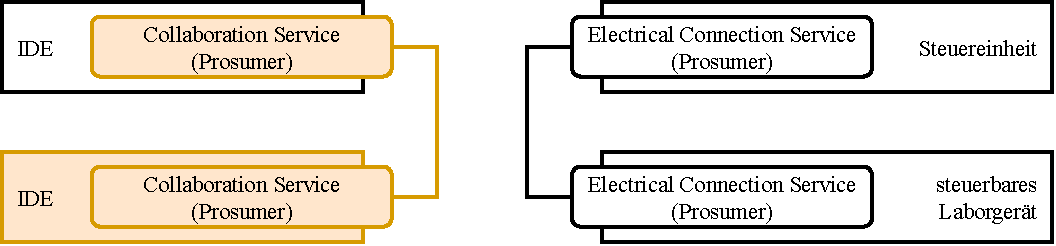
\includegraphics[width=\textwidth]{diagrams/experimentkonfigurationen/Experimentkonfiguration-01.drawio.pdf}
    \caption{Experimentkonfiguration (+ Kollaboration)}
    \label{figure:experimentkonfiguration:kollaboration}
\end{figure}